\documentclass[a4paper,11pt]{article}
\DeclareUnicodeCharacter{2212}{\ensuremath{-}}
\usepackage{jheppub} % for details on the use of the package, please see the JINST-author-manual
\usepackage{lineno}
\usepackage{bm}
% \linenumbers

\arxivnumber{2607.00884} % if you have one

\title{Modeling Falling Backgrounds with Exponential Mixtures}

% Collaborations

%% [A] If main author
%% \collaboration{\includegraphics[height=17mm]{collabroation-logo}\\[6pt]
%%  XXX collaboration}

%% or
%% [B] If "on behalf of"
%% \collaboration[c]{on behalf of XXX collaboration}


% Authors
% The "\note" macro will give a warning: "Ignoring empty anchor...", you can safely ignore it.

%% [A] simple case: 2 authors, same institution
%% \author[1]{A. Uthor\note{Corresponding author.}}
%% \author{and A. Nother Author}
%% \affiliation{Institution,\\Address, Country}

%% or, e.g.
%% [B] more complex case: 4 authors, 3 institutions, 2 footnotes
%% \author[a,b]{F. Irst,\note{Now at another university}}
%% \author[c]{S. Econd,}
%% \author[a,2]{T. Hird\note{Also at Some University.}}
%% \author[c,2]{and Fourth}
%% \affiliation[a]{Institution_1,\\Address, Country}
%% \affiliation[b]{Institution_2,\\Address, Country}
%% \affiliation[c]{Institution_3,\\Address, Country}

\author{Austin Townsend,}
\author{Marc Osherson,}
\author{Mike Hildreth, }
\author{and Stefano Castruccio}
\affiliation{University of Notre Dame, USA}

% E-mail addresses: only for the corresponding author
\emailAdd{atownse2@nd.edu}

\abstract{
Data driven searches for new physics at the LHC often look for localized excesses on smoothly falling background distributions.
Several classes of background models have been considered, including polynomials and other 
parametric families; however, these approaches can require extensive analysis-specific 
development as datasets grow.
In this work, we investigate the finite exponential mixture, defined as a weighted sum of exponential densities with non-negative weights, as a flexible semi-parametric class of functions for approximating falling distributions. The exponential mixture is motivated as a generalization of the positive-shape generalized Pareto distribution from extreme value theory.
Using two published datasets containing 28,619,185 and 5,036 observations, respectively, we show that the finite exponential mixture achieves performance comparable to existing background models.
Finally, in simulation studies with 5,036 observations, we compare the bias, coverage, and spurious signal yield of the exponential mixture with existing background models and find that it exhibits relatively small bias and consistent coverage in the bulk.
}

\DeclareUnicodeCharacter{2009}{\,}
\begin{document}
\maketitle
\flushbottom

\section{Introduction}
\label{sec:intro}

Searching for new particles is a primary focus of high-energy physics, providing the main avenue for probing physics beyond the Standard Model. At the Large Hadron Collider (LHC), these searches can take the form of resonance searches—or "bump hunts"—where high-energy proton collisions are used to produce short-lived, novel states. If a new particle decays into visible final-state products within the detector, and a sufficient number of these observations are recorded, its presence can be identified as a statistically significant localized excess, or "bump," in the reconstructed invariant mass. Standard Model (SM) processes can mimic these decays of new particles; however, in the regions of interest their contributions are often non-resonant. Isolating a genuine signal on top of these sometimes large SM contributions requires an accurate description of the SM expectation.

This paper focuses on background models for resonant searches, where signals are 
represented by localized (resonant) deviations on top of a smooth falling background. The signal 
shapes in non-local (non-resonant) searches vary and require background estimation methods, which 
are out of the scope of this paper.

Background models in resonance searches often rely on mass sidebands (regions 
of the spectrum surrounding a signal window) for identification, and range from 
very flexible to rigid, analysis-specific background models. Flexible models like polynomials are attractive for their universal approximation properties but may need a large number of parameters and can 
be hard to optimize. These models can also be too flexible, fitting the signal or generating nonphysical behaviors in the tails. Previous searches considering polynomials, 
such as those used to discover/measure the Higgs boson properties \cite{CMS_Higgs_Discovery, Aad_2014}, avoid these issues by only fitting a portion of the observed mass spectra near the resonance. Since the Higgs resonance 
occurs within the bulk of the background, the background model is well constrained by the data 
sidebands; however, other analyses extend their search to the extrema of the distributions (tails), where no sidebands are 
available and better extrapolation techniques are required.

Alternatively, analysis-specific background models are often more rigid, avoiding some of the drawbacks that 
come with very flexible models like polynomials. The underlying theory describing the particle 
interactions is complicated enough that there are generally no closed-form expressions for 
describing these backgrounds, though there are some good approximations. A salient example is 
the ``dijet function'', first used in the 1990s by the CDF and D\O\ collaborations and more 
recently by CMS and ATLAS \cite{Harris:2011bh} to describe the invariant mass distribution of 
particle jet pairs in hadron colliders. The terms in this function are motivated by leading 
order quantum chromodynamics (QCD) and the mass dependence of parton distribution 
functions \cite{Harris:2011bh}, but more recently also contain empirically motivated terms. This function works on existing datasets, but 
since it relies on a number of approximations and ad hoc corrections, it is likely to need 
updating as datasets continue to grow in size.

The dijet function has also been applied in other contexts, such as analyses 
involving photons, despite the more complicated background composition 
in those channels. To combat the bias associated 
with the assumption of a particular functional form, more recent analyses \cite{CMS_DP1, 
CMS_high_mass_diphoton, CMS_DP2, CMS_DP3} will often consider a number of background functions 
simultaneously using the discrete profiling method \cite{discrete-profiling}. These functions 
are typically chosen from a larger set of function classes, which can be extended with more 
parameters. In these cases, researchers are typically interested in finding function classes that 
approximate the spectra with the smallest number of parameters. More broadly, there is significant interest in developing generic, 
reusable fitting solutions for resonance searches in high-energy physics, including 
Gaussian-process-based background models \cite{Frate_2017}, and automated symbolic regression \cite{SymbolFit_2025}.

In this paper, we consider finite exponential mixtures as an alternative class of models for smoothly falling backgrounds. Exponential functions and sums of exponentials have been used previously for background modeling; here, we develop a statistical motivation for this model family through its connection to extreme value theory (EVT). Our starting point is the generalized Pareto distribution (GPD), which arises as a limiting model for threshold excesses. Its positive-shape branch also describes excesses of idealized power-law spectra and admits an exact representation as a mixture of exponential densities with gamma-distributed rates. We generalize this representation by allowing a more flexible distribution of rates and approximate it with a finite mixture. This construction provides a statistical motivation for the model family; its suitability over the finite mass intervals considered here is assessed using collision data and simulation studies.

The remainder of this paper is organized as follows. In Section~\ref{sec:emm} we introduce the 
finite exponential mixture and our parameterization. Section \ref{sec:examples} begins with the model selection procedure, implementation details, and global optimization. It is then divided into subsections covering two example datasets: the Run 2 ATLAS dijet dataset (\ref{sec:example1}) and the Run 2 CMS high-mass diphoton dataset (\ref{sec:example2}). In 
Section~\ref{sec:toys} we generate pseudo-datasets using the functions from the Run 2 CMS high-mass diphoton analysis and compare the bias, coverage, and spurious signal of those models 
with the exponential mixture. Section~\ref{sec:discussion} discusses the results, extensions, and areas for future research. Finally the main results are summarized in Section \ref{sec:conclusion}.

\section{Exponential Mixtures}
\label{sec:emm}

A foundational result in EVT, the Pickands–Balkema–de Haan theorem \cite{Picklands_1975, Balkema_Haan_1974}, states that, for a broad class of distributions, the values above a sufficiently high threshold approximately follow a generalized Pareto distribution (GPD). This approximation becomes accurate as the threshold approaches the upper endpoint, which may be finite or infinite, with a scale parameter that generally depends on the threshold. The result motivates considering the GPD as a reference family for falling spectra in high-energy physics: EVT identifies a common limiting form, while the underlying distribution determines how high the threshold must be for that form to provide a useful description. The GPD density is given by:
\begin{equation}
    f_{\mathrm{GPD}}(x \mid u,\sigma,\xi) =
    \begin{cases}
        \displaystyle
        \frac{1}{\sigma}
        \left(1+\xi\frac{x-u}{\sigma}\right)^{-1/\xi-1},
        & \xi \ne 0, \\[6pt]
        \displaystyle
        \frac{1}{\sigma}
        \exp\left(-\frac{x-u}{\sigma}\right),
        & \xi = 0.
    \end{cases}
    \label{eq:gpd}
\end{equation}
Here $u$ is the lower threshold, $\sigma>0$ is the scale parameter,
and $\xi$ is the shape parameter. The variable $x\ge u$ is unbounded
above for $\xi\ge0$, while $\xi<0$ imposes a finite upper limit at
$u-\sigma/\xi$. The sign of $\xi$ distinguishes the three EVT regimes:
a power-law tail for $\xi>0$, an exponential tail for $\xi=0$, and a finite endpoint log-concave distribution for $-1<\xi<0$. For $\xi=-1$ the GPD reduces to the uniform distribution and for $\xi<-1$ the density is increasing. In its decreasing-density range ($\xi>-1$), the GPD transitions from being log-convex ($\xi\geq0$) to log-concave ($\xi\leq0$) passing through the log-linear exponential distribution ($\xi=0$) in between.

In collider applications, the physical upper bound at the center-of-mass energy motivates a negative-shape GPD as a possible description sufficiently close to the endpoint. The range over which endpoint effects become important depends on the spectrum: they may be confined to a narrow interval near the kinematic limit or extend to substantially lower masses. Close to the endpoint, the vanishing spectrum also makes observations increasingly rare. The practical importance of modeling these effects therefore depends on both their extent across the fitted range and the available event count. Over the mass intervals considered by the analyses presented here, the spectra are instead predominantly log-convex, favoring the positive-shape GPD as an alternative reference shape whose power-law behavior is compatible with established parameterizations of non-resonant backgrounds. This compatibility motivates the positive-shape GPD as a starting point, although its specific functional form may be too restrictive to capture variations across the full analysis range. Its representation as an exponential mixture with gamma-distributed rates then suggests a systematic generalization: relaxing the gamma restriction allows for more flexibility.

For the following mixture representations, we measure $x$ relative to the lower threshold, so that $x$ denotes the excess above $u$ and the threshold is located at zero. For $\xi>0$, the GPD has the exponential-mixture representation
$$
f_{\text{GPD}}(x\mid\sigma,\xi>0)
=\int_0^\infty \beta e^{-\beta x}
\pi_\Gamma(\beta\mid a,b) d\beta,
$$
where
$$
\pi_\Gamma(\beta\mid a,b)
=\frac{b^a}{\Gamma(a)}\beta^{a-1}e^{-b\beta},
\qquad
a=\frac{1}{\xi},\qquad b=\frac{\sigma}{\xi},
$$
where $a$ and $b$ are the shape and rate parameters of the Gamma distribution. The exponential case $\xi=0$ corresponds to a rate distribution concentrated at $\beta=1/\sigma$.

This identity motivates replacing the gamma distribution by a general probability distribution $G$ over positive rates:
$$
f_G(x)=\int_0^\infty \beta e^{-\beta x} dG(\beta).
$$
The resulting family contains the positive-shape GPD and exponential reference models while allowing more flexible shapes. Approximating $G$ by a discrete distribution gives the finite exponential mixture density:
$$
f_k(x)=\sum_{i=1}^{k}w_i\beta_i e^{-\beta_i x},
\qquad
w_i\geq0,\quad \sum_{i=1}^{k}w_i=1,\quad \beta_i>0.
$$
The set of rates $\beta_i$ and the corresponding weights $w_i$ provide a finite approximation of the mixing distribution $G$ and likely lack any physical interpretation alone.

Any completely monotone function\footnote{\label{cm_def}A function $f(x)$ is completely monotone if $(-1)^n \frac{d^n}{dx^n}f(x) \geq 0$ for all $n \in {0,1,2,\ldots}$, meaning the function is non-negative, non-increasing, convex, etc.} on $(0,\infty)$ admits a representation as a positive mixture of exponential functions \cite{bernstein} and can be uniformly approximated by finite positive exponential sums on compact intervals contained in $(0,\infty)$ \cite{McGlinn_1978}. Thus, after restricting and normalizing both the target function and the mixture over the same finite analysis interval, finite exponential mixtures can approximate arbitrarily closely any density obtained from a completely monotone function. Familiar examples of completely monotone functions include decreasing exponentials $e^{-\beta x}$, power laws $x^{-\alpha}$, shifted power laws $(1+x/\sigma)^{-\alpha}$, and stretched exponentials $e^{-(x/\sigma)^q}$, for $\alpha,\beta,\sigma>0$ and $0<q\leq1$, on $x>0$. The class of completely monotone functions is closed under addition and multiplication, so positive sums of these functions and products such as exponentially damped power laws also belong to the class. Exponential mixtures therefore provide a common representation for several familiar falling shapes without requiring a particular combination of factors to be specified in advance.

Finally to enforce the condition that the weights $\vec{w}$ sum to 1, the parameters are 
constructed from a set of unconstrained parameters $\vec{v}$ with $k-1$ degrees of freedom 
using the softmax function:
\begin{equation}
\label{softmax}
w_i = \frac{e^{v_i}}{\sum_{j=1}^{k}e^{v_j}} \, ,
\end{equation}
where $v_1=0$ and $v_{i\neq 1} \in (-\infty,\infty)$.

\section{Examples} \label{sec:examples}

The examples in this section are selected from public datasets available on \href{https://www.hepdata.net/}{\texttt{HEPData}} which is an online repository for publication-related high energy physics data \cite{Maguire_2017}. We select both large and small datasets corresponding to two jet and two photon final states to test the robustness of the method to dataset size and background composition.

In the following sections, we compare the finite exponential mixture to the original methods. The model parameters are estimated via maximum likelihood using the Python interfaces to \texttt{RooFit}~\cite{RooFit} and \texttt{ROOT}~\cite{ROOT}, which are commonly used in high-energy physics.

Numerical optimization is performed with \texttt{MINUIT} and the \texttt{MIGRAD} algorithm~\cite{Minuit2}. Because the likelihood is non-convex in the mixture parameters, fits to the observed datasets and to each independently generated pseudo-dataset use multiple randomized starting points. The additional fits to bootstrap resamples described in Section~\ref{sec:coverage} do not repeat this random-restart search. At each starting point, minimization is repeated until the returned status is 0 (successful minimization), 1 (the covariance matrix was forced positive definite), or 2 (the Hessian calculation was invalid), or until a prescribed limit on the number of fit calls is reached. Among the accepted results, the parameter values yielding the lowest negative log-likelihood are retained.

We permit these covariance-related warnings because our primary interest is the fitted density rather than the individual component parameters or their Hessian-based uncertainties. Components with nearly equal rates can exchange weight with little change in the density, while the rate of a component with negligible weight may be poorly determined. An unreliable parameter covariance matrix therefore need not imply an equally unstable density estimate. Nevertheless, the associated flat likelihood directions may impede optimization, and this acceptance criterion does not establish that the minimum has been located accurately. The restart and fit-call budgets are specified separately for each example and are heuristic implementation choices that do not certify global optimality. For ease of implementation, the rates are standardized relative to the single-exponential estimate $1/(\mathbb{E}(X)-X_{\min})$, and each rate is capped at 50 times that reference value to prevent overfitting at the lower 
boundary.

For each dataset, a sequence of models with increasing numbers of exponential components is fit, and the preferred value of $k$ is chosen by the Akaike information criterion (AIC), while also recording the Bayesian information criterion (BIC)
\footnote{The AIC and BIC are the penalized likelihood criteria $\mathrm{AIC}=-2\ell_{\max}+2p$ 
and $\mathrm{BIC}=-2\ell_{\max}+p\log n$, where $\ell_{\max}$ is the maximized log-likelihood, $p$ is the number of free parameters, and $n$ is the sample size. Both balance the goodness of fit against model complexity, but BIC penalizes additional parameters more strongly when $n$ is 
large and therefore tends to prefer simpler models.
} for comparison following the discussion of the mixture-model 
selection in McLachlan and Peel~\cite{finite-mixture-models}. The justification for preferring AIC in these studies is deferred to Sections~\ref{sec:toys} and~\ref{sec:discussion}. Both criteria can be expressed as thresholds on the improvement in the maximized log-likelihood: adding one exponential component introduces two free parameters, so AIC favors the larger model when $2\Delta\ell>4$, whereas BIC requires $2\Delta\ell>2\log n$. Finite mixtures can violate the regularity assumptions underlying standard likelihood-ratio tests and the usual theoretical justifications of information criteria. We therefore treat AIC and BIC as practical selection rules and assess their performance through simulation studies.

In \texttt{RooFit}, the normalization of the density depends on the defined observable range, which has consequences for model selection. Unless noted otherwise, we take $X_{\max}=10$~TeV, below the 13~TeV center-of-mass energy. The remaining dataset-specific choices, including whether the likelihood is binned or unbinned and the exact restart settings, are given in the corresponding subsections.

\subsection{ATLAS Dijet Spectrum} \label{sec:example1}

The dataset used in this section was collected by the ATLAS experiment at the LHC during the 
Run~2 data-taking period, spanning from 2015 to 2018.
The publication, Ref. \cite{ATLAS_dijet}, uses several signal regions defined by the half rapidity separation between the two leading jets $y^*= (y_1 - y_2)/2$, where $y_1$ and $y_2$ are the rapidities of the leading and subleading jets. For this example, we use the signal region defined by $|y^*|<0.6$. 

The dijet function used in this analysis is given by:
\begin{equation}
f_D(x) = p_0(1-x)^{p_1}/x^{p_2+p_3\log x},
\end{equation}
where $x=m_{jj}/\sqrt{s}$ for the dijet invariant mass $m_{jj}$ and center-of-mass energy 
$\sqrt{s}=13$~TeV.
Simpler versions of this function have been used in the past with $p_3=0$, but as datasets grow, these parameterizations must be extended. Because of this concern, ATLAS uses a sliding window fit method \cite{ATLAT_Dijet_sliding_window}, which reduces the fit range to the vicinity of the signal hypothesis being tested. For simplicity, we do not replicate this technique; instead fitting the entire spectrum at once.

With the exception of the $x^{p_3\log x}$ term, the components of the dijet function correspond to distinct physical phenomena: the finite energy threshold ($(1-x)^{p_1}$) and approximate scale invariance ($x^{-p_2}$). At sufficiently high energies, Standard Model quarks can be treated as massless, yielding a theory that is approximately scale-invariant up to the running of the strong coupling constant $\alpha_s$. While a finite exponential mixture is not inherently scale-invariant, it can approximate scale-invariant distributions like $x^{-p_2}$ (for $p_2>0$) arbitrarily closely as the number of mixture components increases. Furthermore, although the exponential mixture does not explicitly model the finite energy threshold, it can still provide a reliable approximation depending on where the upper tail is truncated.

The dataset available on \texttt{HEPData} is binned. In high-energy physics, datasets can be very large, making fits to the unbinned data time-consuming. In such cases, it is common practice to bin the data finely enough to retain information, while coarsely enough that the fits converge in reasonable times. In this analysis the bin widths are determined by the dijet invariant mass resolution, which broadens at higher 
values. The binned likelihood is given by the product of Poisson probabilities,
\begin{equation}
L(\theta)=\prod_b \operatorname{Pois}\left(n_b\mid Np_b(\theta)\right),
\end{equation}
where $n_b$ is the observed count in bin $b$, $N=\sum_b n_b$ is the observed total event count, and
\begin{equation}
p_b(\theta)=\int_{b^-}^{b^+}f(m;\theta)dm
\end{equation}
is the probability of an event falling in that bin. Here $b^-$ and $b^+$ denote the bin edges, and $f(m;\theta)$ is normalized over the fitted mass range. The expected bin count is therefore $Np_b(\theta)$. We fix the total normalization to the observed event count $N$ and fit only the shape parameters. Because the finite exponential mixture is a linear combination of exponential functions, $p_b$ analytically evaluates to a simple closed form. Exact integrals eliminate the need for computationally intensive numerical integration routines during minimization.

The binning provided on \texttt{HEPData} includes only a single small-width bin following the 
last bin with non-zero entries.
Because model selection depends on the upper threshold of the fit, an additional bin with zero 
entries extending to 10~TeV is appended to constrain upper tail behavior.
For the dijet example, we use 80 randomized starting points and allow at most 30 fit calls per starting point. These settings specify the computational budget used in this study; they are not established as optimal or generally sufficient.

\begin{figure}
    \centering
    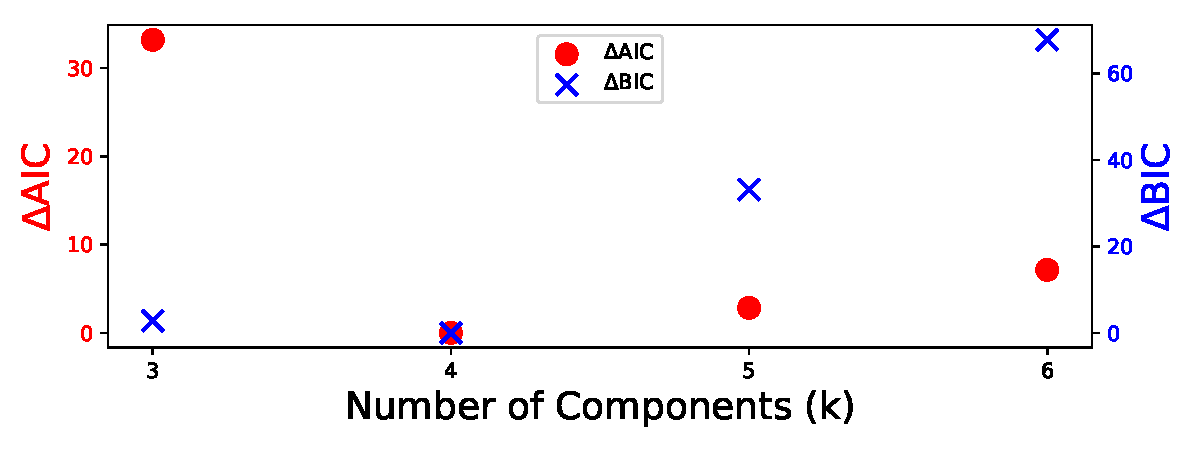
\includegraphics[width=\linewidth]{figures/dijet_model_selection.pdf}
    \caption{Relative AIC (red dot) and BIC (blue x) scores for exponential mixtures on the ATLAS dijet 
    dataset for $k=3,4,5,6$ mixture components. The relative AIC/BIC is given by $\Delta\text{IC}_i=\text{IC}_i-\min(\text{IC})$ where $\text{IC}$ is either AIC or BIC.}
    \label{fig:dijet_AIC_BIC}
\end{figure}

\begin{figure}
    \centering
    
\includegraphics[width=\linewidth]{figures/dijet_fit.png}
    \caption{Fit of the dijet function and exponential mixture to the ATLAS Run~2 dijet dataset 
    (top) and normalized residuals (bottom).}
    \label{fig:dijet_fit}
\end{figure}

\begin{table}
\centering
\begin{tabular}{lccccc}
\hline
Model & $\chi^2$ & $\chi_\nu^2$ & $\nu$ & $\Delta$AIC & $\Delta$BIC \\
\hline
Dijet Function            & 95.8 & 1.29 & 74 & 0.66 & 0 \\
Exponential Mixture (AIC) & 89.2 & 1.27 & 70 & 0 & 60 \\
\hline
\end{tabular}
\caption{Goodness-of-fit metrics for the dijet function and finite exponential mixture chosen by AIC ($k=4$) fit to the 
Run~2 ATLAS dijet data. For the $\chi^2$ calculation, low-event-count bins are merged until they contain at least 30 observations and $\nu$ is the number of degrees-of-freedom.}
\label{tab:dijet_AIC_BIC}
\end{table}

Figure~\ref{fig:dijet_AIC_BIC} compares the AIC and BIC scores for exponential mixtures of varying complexity to determine the best fit for the dijet dataset. In this case AIC and BIC agree, the best model has four components. The goodness-of-fit metrics are shown in Table~\ref{tab:dijet_AIC_BIC} where we compare between the dijet function and the exponential mixture. The exponential mixture achieves a slightly smaller AIC and $\chi^2$ but uses more parameters.
Figure~\ref{fig:dijet_fit} shows the fit of the dijet function and the 4-component exponential mixture to the dijet dataset.
The residuals show that the two functions provide similar estimates throughout the mass range.

\subsection{CMS High-Mass Diphoton Spectrum} \label{sec:example2}

The dataset considered in this section is the Run~2 dataset published by CMS in the high-mass two-photon final state \cite{CMS_high_mass_diphoton}.
Only the barrel--barrel sample (EBEB, $n=5,036$) is used here.

The background estimate for this analysis uses the discrete profiling method with the following 
functions:
 \begin{subequations}\label{eq:diphoton_fns}
\begin{align}
    f_1(x)&=p_0x^{p_1+p_2\log(x)}, \label{eq:diphoton_f1} \\
    f_2(x)&=p_0e^{p_1x}x^{p_2}, \label{eq:diphoton_f2} \\
    f_3(x)&=p_0(1+xp_1)^{p_2}, \label{eq:diphoton_f3} \\
    f_4(x)&=p_0(1+xp_1)^{p_2+p_3x} \label{eq:diphoton_f4}
\end{align}
\end{subequations}
where $x\equiv m_{\gamma\gamma}/\sqrt{s}$, $m_{\gamma\gamma}$ is the invariant mass of the 
two-photon system, and $\sqrt{s}=13$~TeV is the center-of-mass energy.
These functions are chosen from extendable classes of functions built using power laws, exponentials, and threshold-shifted polynomials, most of which are also used in the dijet function. For model specification, the primary analysis references \cite{CMS_DP1}, where the explicit criterion is to choose the lowest-order function yielding a $\chi^2$ goodness-of-fit $p$-value greater than 5\% for each functional family.

With the published parameter estimates on \texttt{HEPData} it can be shown that $f_2$ and $f_3$ are completely monotone functions.
The first function $f_1$ has completely monotone components, but the term $x^{p_2 \log(x)}$ is not; most departures from complete monotonicity are found at low $x$. The derivatives of $f_4$ are more complicated, with no guarantee of complete monotonicity, though it is possible for the published parameter estimates.

While the official \texttt{HEPData} entry provides a binned dataset, the unbinned data were 
obtained from the CMS collaboration upon request.
In this case, the likelihood is given by:
\begin{equation}
    \mathcal{L}(\vec\theta) = \prod_{i=1}^N p(x_i|\vec\theta),
\end{equation}
where $\vec\theta$ are the model parameters and $p$ is the probability density function. For the diphoton example, we use 20 randomized starting points and allow at most 5 fit calls per starting point.

\begin{figure}
    \centering
    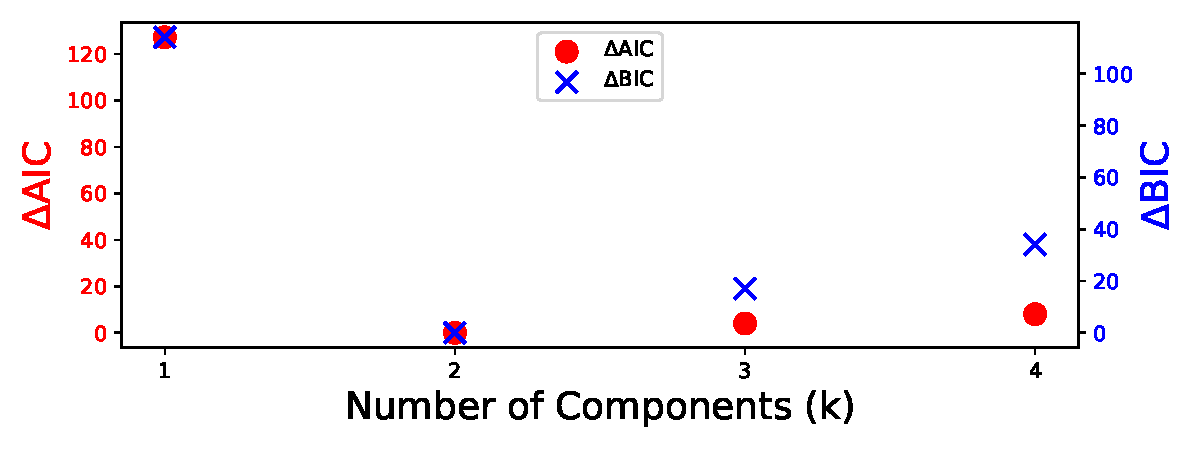
\includegraphics[width=\linewidth]{figures/diphoton_model_selection.pdf}
    \caption{Relative AIC (red dot) and BIC (blue x) scores for exponential mixtures on the CMS 
    high-mass diphoton dataset for $k=1,2,3,4$ mixture components. The relative AIC/BIC is given by $\Delta\text{IC}_i=\text{IC}_i-\min(\text{IC})$ where $\text{IC}$ is either AIC or BIC.}
    \label{fig:diphoton_model_selection}
\end{figure}

\begin{figure}[h]
    \centering
    
\includegraphics[width=\linewidth]{figures/diphoton_fit.png}
    \caption{Fit of the original functions and exponential mixture (AIC) to the CMS high-mass diphoton dataset (top) and normalized residuals (bottom). For visualization, the data and density functions are binned.}
    \label{fig:diphoton_fit}
\end{figure}

\begin{table}[h]
\centering
\begin{tabular}{lccccc}
\hline
Model & $\chi^2$ & $\chi^2_\nu$ & $\nu$ & $\Delta$AIC & $\Delta$BIC \\
\hline
$f_1$ & 54.2 & 0.93 & 58 & 2.3 & 1.6 \\
$f_2$ & 53.5 & 0.92 & 58 & 0.8 & 0.0 \\
$f_3$ & 54.7 & 0.94 & 58 & 3.3 & 2.5 \\
$f_4$ & 53.4 & 0.94 & 57 & 2.6 & 8.4 \\
Exponential Mixture (AIC) & 50.6 & 0.89 & 57 & 0.0 & 5.7 \\
\hline
\end{tabular}
\caption{Goodness-of-fit metrics for $f_1$, $f_2$, $f_3$, $f_4$, and the finite exponential mixture chosen by AIC ($k=2$) 
fit to the Run~2 CMS high-mass diphoton data. For the $\chi^2$ calculation, low-event-count 
bins are merged until they contain at least 30 observations and $\nu$ is the number of degrees-of-freedom.} 
\label{tab:diphoton_AIC_BIC} 
\end{table}

Figure~\ref{fig:diphoton_model_selection} shows that both AIC and BIC prefer a two-component exponential mixture and in Table~\ref{tab:diphoton_AIC_BIC} we compare the goodness-of-fit between the four original functions and the two-component exponential mixture. We see that the exponential mixture fit quality is comparable to that of the original functions, with the smallest $\chi^2$ and the smallest AIC. The fits of all four original functions and the exponential mixture are shown in Figure~\ref{fig:diphoton_fit}; the dataset is binned for visualization.

\section{Simulation Studies}\label{sec:toys}

In this section, the performance of the exponential mixture is quantified by fitting pseudo-datasets generated from each of the functions in eq.~\eqref{eq:diphoton_fns}. In each case, the data-generating parameters are obtained via maximum likelihood estimation (MLE) on the CMS high-mass diphoton dataset. The number of exponential components is determined independently for each pseudo-dataset, and results are shown for both AIC and BIC model selection metrics. For each independently generated pseudo-dataset, the candidate mixture orders are fitted using the random-restart procedure before applying AIC or BIC. Agreement is quantified in terms of bias, coverage, and spurious signal yield.

\subsection*{Bias}

We quantify bias relative to the statistical uncertainty in the density estimate obtained using the data-generating model. This relative bias, $B(x)$, is defined as
\begin{equation}
B(x)=\frac{1}{T\sigma(x)}
\sum_{t=1}^{T}\left[f(x\mid\hat{\beta}t)-f{\mathrm{true}}(x)\right],
\end{equation}
where $f_{\mathrm{true}}(x)$ is the density used to generate the pseudo-datasets, $f(x\mid\hat{\beta}_t)$ is the fitted density for pseudo-dataset $t$, and $\sigma(x)$ is the standard deviation across density estimates obtained by fitting the data-generating model to those pseudo-datasets. Thus, $B(x)$ expresses the average density bias in units of this reference statistical uncertainty.

Figure~\ref{fig:bias} shows the relative bias of the exponential mixture for each of the four data-generating functions in Eq.~(3.4), with fits using the remaining three functions shown for comparison. We assess these curves primarily through the magnitude and mass dependence of the relative bias. When bias magnitudes are comparable, more frequent zero-crossings indicate that departures from the true density are less persistently of one sign across the mass range, consistent with greater flexibility in matching its shape; crossing counts alone do not establish better performance. The AIC-selected exponential mixture combines more frequent zero-crossings with smaller relative bias than the BIC-selected mixture, remaining mostly within one reference standard deviation of zero. It also achieves among the smallest relative biases among competing models, though it uses more parameters than most. In the high-mass tail, the bias becomes smaller relative to the spread of density estimates obtained with the data-generating model.

\begin{figure}[h!]

\includegraphics[width=\textwidth]{figures/bias.png}
\caption{Relative bias ($B(x)$) of the estimated density for various functions. Each row represents 
approximately $T=5000$ pseudo-datasets simulated from the data-generating model with $n=5{,}036$ entries. 
The shaded regions represent the $\pm1$ standard deviation band for estimates using the data-generating model.}
\label{fig:bias}
\end{figure}

\subsection*{Coverage}\label{sec:coverage}

Coverage is evaluated by calculating how often the true density falls within the estimated pointwise confidence intervals across independently generated pseudo-datasets. Constructing these intervals requires accounting for the joint dependence among fitted parameters and their nonlinear mapping to the density. When a local quadratic approximation to the likelihood is adequate, the estimated parameter covariance matrix can be used for approximate uncertainty propagation. In finite exponential mixtures, however, individual component parameters can be poorly constrained even when the combined density is comparatively well constrained. Components with nearly equal rates can exchange weight with little change in the density, while the rate of a component with negligible weight is weakly constrained by the data. These configurations can produce nearly flat likelihood directions, making the quadratic approximation unreliable. We therefore use the non-parametric bootstrap \cite{Efron_1986} to construct pointwise confidence intervals directly from an ensemble of fitted densities.

For each independently generated pseudo-dataset $D$, we draw $B$ bootstrap resamples of the same size by sampling its observations with replacement. Each candidate mixture order is refitted to every resample, starting from the parameter estimates obtained for that order by the random-restart procedure applied to $D$. The random-restart search is not repeated within each resample. The number of components $k$ is selected again using the same information criterion, so the ensemble includes variation associated with both parameter estimation and model selection. At each mass value $x$, the pointwise confidence interval is defined by the $100\alpha/2$ and $100(1-\alpha/2)$ percentiles of the fitted bootstrap densities. We use $\alpha=0.05$, corresponding to the 2.5th and 97.5th percentiles.

These intervals reflect variability estimated from each pseudo-dataset, but resampling does not automatically correct bias from background misspecification or model selection. Their nominal 95\% confidence level therefore does not guarantee 95\% coverage. To assess their actual coverage, we repeat the full interval-construction procedure across independently generated pseudo-datasets and record how often the resulting intervals contain the known true density.

The coverage of model $f$ for the true density $f_t$ is estimated as: 
\begin{equation}
    C(x|f,f_t,T,B) = \frac{1}{T}\sum_{i=1}^T I(x|D_i)
\end{equation}
where $T$ is the number of pseudo-datasets ($n=5{,}036$), $B$ is the number of bootstrap resamples, and 
$I(x|D)$ is the indicator function:
\begin{equation}
    I(x|D) =
    \begin{cases}
        1, & \text{if } f_{t}(x) \in \mathrm{CI}_B(x|f,D), \\
        0, & \text{otherwise,}  
    \end{cases}
\end{equation}
where $\mathrm{CI}_B(x)$ is the bootstrap confidence interval with $B$ resamples.

Figure~\ref{fig:coverage} shows the estimated pointwise coverage, calculated at each mass as the fraction of the $T=400$ independently generated pseudo-datasets whose fitted confidence interval contains the true density. The AIC-selected exponential mixture generally achieves coverage close to the nominal 95\% level across the bulk of the fitted spectrum, with departures near the lower boundary and increasing undercoverage in the high-mass tail. Its coverage is generally closer to nominal than that of the BIC-selected mixture.

The finite number of pseudo-datasets introduces fluctuations in these coverage estimates. For an underlying coverage of 95\%, the standard deviation of the measured fraction is $\sqrt{0.95(1-0.95)/400}\simeq0.011$, corresponding to approximately 1.1 percentage points. Small departures from the nominal level should therefore be interpreted in light of this statistical precision. Estimates at different masses are also correlated because they are obtained from the same pseudo-datasets.



\begin{figure}[h!]

\includegraphics[width=\textwidth]{figures/coverage.png}
\caption{Coverage of the estimated density for various functions. Each row represents $T=400$ 
pseudo-datasets simulated from the data-generating model with $n=5{,}036$ entries. The 95\% confidence 
interval is calculated using $B=1000$ bootstrap resamples.}
\label{fig:coverage}
\end{figure}

\subsection*{Spurious Signal}
The spurious signal is the signal yield extracted from a signal-plus-background fit when no signal is present. It measures the extent to which background mismodeling can produce an apparent signal, providing a diagnostic of potential bias in resonance searches. We evaluate this using pseudo-data generated from known background distributions. We fit each pseudo-dataset with a signal-plus-background model
\begin{equation}
f(x;\mu,\theta)=(1-\mu)b(x;\theta)+\mu s(x),
\end{equation}

where \(b(x;\theta)\) is the normalized background density and \(s(x)\) is a Gaussian signal density normalized over the fit range, with fixed mean and width for each signal hypothesis. The parameter \(\mu\) is the signal fraction, with \(\mu=0\) corresponding to the background-only hypothesis. We also allow negative values of \(\mu\), subject to the total density remaining non-negative, to identify both apparent excesses and deficits.

We quantify the spurious signal using the signed profile likelihood statistic
\begin{equation}
r_0 = \operatorname{sign}(\hat{\mu})\sqrt{-2\ln\lambda(0)},
\end{equation}
where $\lambda(\mu)$ is the profile likelihood ratio defined in Eq.~(7) of Ref.~\cite{Cowan_2011}. Its sign distinguishes apparent excesses from deficits. Under the Wald approximation,
$-2\ln\lambda(0)\approx\hat{\mu}^2/\sigma_\mu^2$, so $r_0$ reduces to the commonly used ratio $\hat{\mu}/\sigma_\mu$ (see Eqs.~(17)--(18) of Ref.~\cite{Cowan_2011}). The uncertainty $\sigma_\mu$ is typically estimated from the inverse Hessian of the negative log likelihood, whose inversion can be unstable when the likelihood is flat. Using $r_0$ avoids this explicit covariance-matrix inversion and does not require a local quadratic approximation to the likelihood, although its interpretation as a Gaussian significance still relies on asymptotic approximations.

For each pseudo-dataset, the mixture order $k$ is selected using the background-only fit and is then held fixed when evaluating the profile likelihood ratio. The continuous background parameters are reoptimized both with the signal fraction fixed to zero and with it allowed to float. The resulting statistic therefore compares the background-only and signal-plus-background hypotheses within the same selected mixture order.

The Gaussian signal model has a standard deviation ranging from 25 GeV at the lowest mass hypothesis (500 GeV) to 60 GeV at the highest (2000 GeV). For each of the four data-generating functions in Eq.~\eqref{eq:diphoton_fns}, signal-plus-background fits are performed on 1000 pseudo-datasets at each mass hypothesis. The AIC- and BIC-selected exponential mixtures are compared with fits using the corresponding data-generating background model.

Figure~\ref{fig:spurious} shows the median and central 68\% interval of $r_0$ across the pseudo-datasets, with intervals displayed for the AIC-selected mixture and the data-generating model. The median values for the AIC-selected mixture are generally small relative to the spread obtained with the data-generating model, and its central intervals generally include zero. These intervals describe variation across pseudo-datasets rather than confidence intervals from individual fits. Negative values indicate that the fitted background over-predicts the density in the signal region, while positive values indicate under-prediction. The mass range is restricted to 2000 GeV to avoid numerical underflow encountered in sparsely populated regions. The pattern of spurious signal is broadly consistent with the density bias shown in Figure~\ref{fig:bias}: regions of background under-prediction correspond to positive fitted signal fractions, and vice versa.

\begin{figure}
    \centering
    
\includegraphics[width=0.9\linewidth]{figures/spurious_signal.png}
    \caption{Signed profile likelihood statistic $r_0$ for signal-plus-background fits using the data-generating background models and the exponential mixtures. Each point represents the median over $T=1000$ background-only pseudo-datasets; bands show the central 68\% interval and are displayed only for the data-generating model and the AIC-selected exponential mixture. Each subplot corresponds to a different data-generating model.} 
    \label{fig:spurious}
\end{figure}


\section{Discussion} \label{sec:discussion}

The present work investigates exponential mixtures as a flexible framework for modeling smoothly falling backgrounds in high-energy physics. The exponential-mixture representation of the positive-shape GPD motivates the construction, while complete monotonicity defines the shape restriction retained by the generalized model. This restriction is a modeling assumption whose suitability must be assessed for the spectrum and fit range under consideration. In the ATLAS dijet and CMS diphoton examples, finite exponential mixtures provide fits comparable to the reference parameterizations despite substantial differences in dataset size and background complexity.

Our starting point is the positive-shape GPD, which has an exponential-gamma mixture representation. We relax the gamma restriction to allow a more general distribution of rates and for practical reasons we approximate the resulting mixture with a finite number of components. The number of components therefore controls the resolution of this approximation; it is not assumed to represent a fixed physical order of the background. We favor retaining as much flexibility as the data can meaningfully constrain, while limiting additional parameters that offer little improvement and make optimization more difficult.

The simulation studies support this preference for flexibility between the metrics considered. At the sample size considered ($n=5036$), AIC selects larger mixtures than BIC, yielding more zero-crossings in the bias curves, smaller bias, better coverage, and smaller spurious signal. A plausible explanation is that the complete-monotonicity constraint limits the ability of additional components to reproduce statistical fluctuations, so that their main benefit in these studies is to reduce underfitting. AIC provides acceptable performance in this setting, but these findings motivate investigating criteria that permit greater complexity or assess more directly whether the data meaningfully constrain additional parameters.

Additional background flexibility can reduce sensitivity to a resonant signal, although this tradeoff should be assessed alongside robustness to background misspecification. Exponential mixtures remain completely monotone as components are added, restricting their ability to reproduce localized resonant structure. These constraints do not eliminate partial signal absorption: when a localized deviation is compatible with an admissible variation in the background, increased uncertainty in the extracted signal yield can reflect the limited information available to distinguish these explanations. The background-only studies presented here favor the AIC-selected mixtures over the BIC-selected mixtures in terms of the bias, coverage, and spurious signal considered. These results support retaining additional background flexibility for density estimation, but do not establish the preferred complexity for a resonance search. Determining that choice requires assessing signal recovery and discovery power alongside control of false-positive rates.

The applicability of this framework nevertheless depends on the spectrum and fit range. Although smoothly falling energy spectra away from SM resonances are often expected to be monotone, complete monotonicity\footref{cm_def} is a stronger condition. In particular, it does not describe the turn-on near a lower threshold or the vanishing spectrum at a finite upper endpoint. Analyses typically mitigate turn-on effects by imposing a sufficiently high lower threshold; alternatively, these effects can be modeled independently and combined with the exponential mixture. Near the upper endpoint, a negative-shape GPD may provide an appropriate description, while a truncated exponential mixture may still approximate the spectrum over an interval where endpoint effects are modest. A more complete model could incorporate the endpoint explicitly. For example, one could retain the $(1-m_{jj}/\sqrt{s})^{p_1}$ factor of the traditional dijet function while replacing its power-law component with an exponential mixture.

Even within a suitable fit range, some aspects of regularization and range selection require further study. Near the lower threshold, steeply falling components with small weights can fit local fluctuations. We therefore parameterize the rates relative to the single-exponential estimate $1/(\mathbb{E}(X)-X_{\min})$ and impose an upper bound of 50 times this reference rate. This choice limits such behavior, but a more principled regularization criterion remains desirable. Model selection also depends on the upper fit threshold because the likelihood normalization depends on the fitted range, as implemented in \texttt{RooFit}. Including a substantial zero-event region above the last observation constrains the tail, but the extent of this region remains an analysis choice whose influence warrants further investigation.

Optimization remains a practical limitation of the present implementation. The likelihood is non-convex in the mixture parameters and can contain nearly flat directions when components have similar rates or negligible weights. Random restarts reduce dependence on initialization, but the finite search used here does not certify that the global maximum has been reached. The restart and retry budgets are heuristic, and their sufficiency across datasets and model complexities has not been established. Residual optimization error can also affect model selection when competing information-criterion values are close. An adaptive stopping criterion could help allocate computational effort according to the observed progress of the optimization, reducing reliance on manually chosen budgets while providing a reproducible rule for terminating the search. Beyond refining the current restart procedure, alternative strategies such as split-and-merge methods developed for Gaussian mixtures \cite{split-and-merge} warrant investigation for their potential to improve optimization reliability and efficiency in exponential mixtures.

Alternative parameterizations may also help address these computational difficulties. An ordered-rate parameterization, in which the fit parameters are the smallest rate, the positive differences between successive rates, and the mixture weights, removes the equivalent solutions arising from permutations of component labels without restricting the flexibility of the model. Ordering alone does not resolve weak identifiability when rates nearly coincide, but imposing a minimum separation between adjacent rates can regularize the fit by preventing components from having nearly identical shapes. Such a restriction introduces an additional choice that may improve numerical stability at the expense of flexibility.

Separately, alternative basis functions or more specialized parameterizations may offer statistical advantages. If the data-generating distribution is completely monotone, finite exponential mixtures can approximate it increasingly closely as the number of components grows, but this does not imply that they provide the most efficient representation at a finite sample size. In the diphoton example, $f_2$ achieves a slightly larger AIC (and a smaller BIC) than the exponential mixture (see Table~\ref{tab:diphoton_AIC_BIC}), and for the published parameter estimates $f_2$ has an exponential mixture representation. This suggests that useful structure within the mixture class may be captured more efficiently by parameterizations tailored to particular spectra.

Further simulation studies could more fully characterize the performance and applicability of the exponential mixture framework. Signal-injection and sensitivity studies could assess performance in the presence of a signal and evaluate how the choice of background model and its complexity affects discovery potential and exclusion limits. Studies at larger and smaller sample sizes would help establish whether the results obtained with 5,036 observations extend to other regimes. Although the fit to the observed dijet spectrum demonstrates applicability to a much larger dataset, it does not establish the corresponding repeated-sample performance. Extending the simulations to other background shapes would further clarify how broadly the observed performance holds.

Exponential mixtures provide a systematic way to introduce background flexibility while preserving explicit assumptions about the shape of the spectrum. Their connection to EVT motivates the model class, while the finite mixture representation allows its complexity to adapt to the information available in a given dataset. The results presented here support further development and validation of this approach for resonance searches. Whether used directly over a suitable fit range or incorporated into a broader model that accounts for turn-on and endpoint effects, exponential mixtures offer a common foundation for describing smoothly falling backgrounds across diverse analyses.

\section{Conclusion} \label{sec:conclusion}

The finite exponential mixture has been considered as an alternative approach to modeling 
smoothly falling backgrounds in high-energy physics, motivated by EVT.
This class provides a flexible semi-parametric basis for approximating falling distributions 
without committing to an analysis-specific functional form. In the ATLAS dijet and CMS 
high-mass diphoton examples, the exponential mixture gives fits comparable to existing methods despite substantial differences in dataset sizes and background complexity.
In pseudo-dataset studies based on the functions used by the published diphoton search \cite{CMS_high_mass_diphoton}, the AIC-selected exponential mixture has small bias, good coverage in the bulk, and small spurious signal.

These results suggest that the finite exponential mixture is a promising, statistically motivated general-purpose basis for modeling falling backgrounds in resonant searches. The model is broad enough to adapt to different, smoothly falling spectra while remaining subject to an explicit complete-monotonicity constraint; however, it exhibits clear limitations. Because the distributions of interest are not guaranteed to be completely monotone, non-completely-monotone effects—such as threshold turn-on behavior, finite-energy cutoffs, and other process-specific features—may need to be modeled separately. Furthermore, because performance depends on heuristics for model selection, fit range, and optimization, further work in these areas and in the treatment of non-completely-monotone effects will be essential to improving the performance and generality of this reusable model class.

\section*{Data Availability}
The dataset(s) analyzed during the current study are publicly available on \href{https://www.hepdata.net/}{HEPData}, see Ref. \cite{Maguire_2017} for more information. These data can be accessed at: \url{https://doi.org/10.17182/hepdata.91126} for the ATLAS dijet dataset and \url{https://doi.org/10.17182/hepdata.150677} for the CMS diphoton dataset. The unbinned CMS diphoton dataset used in this study was provided by the CMS collaboration and can be found in the repository given in the next section.

The published binned ATLAS dijet and CMS diphoton datasets are publicly available on \href{https://www.hepdata.net/}{HEPData}~\cite{Maguire_2017} at \url{https://doi.org/10.17182/hepdata.91126} and \url{https://doi.org/10.17182/hepdata.150677}, respectively. The unbinned CMS diphoton dataset used in this study was provided by the CMS collaboration and is available in ROOT format in the accompanying code repository, linked in the Code Availability section.

\section*{Code Availability}
The custom code used to generate the results and figures in this manuscript is available on GitHub at: \url{https://github.com/atownse2/26.Townsend.expmix.unpublished}.

% Bibliography

%% [A] Recommended: using JHEP.bst file
\bibliographystyle{JHEP}
\bibliography{main.bib}

%% or
%% [B] Manual formatting (see below)
%% (i) We suggest to always provide author, title and journal data or doi:
%% in short all the informations that clearly identify a document.
%% (ii) please avoid comments such as "For a review'', "For some examples",
%% "and references therein" or move them in the text. In general, please leave only references in the bibliography and move all
%% accessory text in footnotes.
%% (iii) Also, please have only one work for each \bibitem.

\end{document}
